\documentclass{book}



% Packages
\usepackage{amsmath}
\usepackage[utf8]{inputenc} % Encoding
\usepackage[T1]{fontenc}  % Font encoding
\usepackage[colorlinks=true,linkcolor=blue,urlcolor=blue,citecolor=blue]{hyperref}     % Hyperlinks
\usepackage{geometry}     % Page layout
\usepackage{graphicx}
\usepackage{listings}     % Code listings
\usepackage{xcolor}       % Colors for code
\usepackage{tcolorbox} % Add this to your preamble

% Page layout
\geometry{margin=1in}

% Functions
\tcbset{
    attentionbox/.style={
        colback=red!5, % Background color
        colframe=red!75!black, % Border color
        coltitle=black, % Title color
        boxrule=0.8mm, % Thickness of the border
        left=2mm, % Left padding
        before skip=5mm, % Space before the box
        after skip=5mm, % Space after the box
        sharp corners, % Sharp corners for the box
        fonttitle=\bfseries, % Bold title font
        attach boxed title to top left={yshift=-2mm,xshift=2mm}, % Title position
        boxed title style={
            size=small,
            colback=red!50,
            colframe=red!75!black,
            sharp corners,
        },
    }
}

% % Code formatting
\lstset{
    language=Python,
    basicstyle=\ttfamily\fontsize{9}{10}\selectfont,
    breaklines=true,
    frame=single,
    keywordstyle=\color{blue},
    commentstyle=\color{green!70!black},
    stringstyle=\color{red},
    showstringspaces=false,
    numbers=left,
    numberstyle=\tiny\color{gray},
    stepnumber=1,
    numbersep=10pt,
    xleftmargin=5mm,
}

\title{Interactive UI Tutorial}
\author{The International BioBrillouin Society}
\date{\today}

\begin{document}

\maketitle

\tableofcontents

\chapter{Introduction}
Welcome to the interactive UI tutorial. This book will guide you through the steps to create and use the UI effectively.

The HDF5\_BLS package is a Python library for handling Brillouin light scattering (BLS) data and converting it into a standardized HDF5 format. The library provides functions to open raw data files, store their properties, convert them into a Power Spectral Density (PSD) and analyze the PSD with a standardized treatment protocol. The library is currently compatible with the following file formats:
\begin{itemize}
    \item \textbf{*.dat} files: spectra returned by the GHOST software or obtained using Time Domain measurements
    \item \textbf{*.tif} files: an image format that can be used to export 2D detector images.
    \item \textbf{*.npy} files: an arbitrary numpy array
    \item \textbf{*.sif} files: image files obtained with Andor cameras
\end{itemize}

The package comes with a graphical user interface (GUI) that allows users to easily open, edit, and save data. This interface is the preferred way to use the package and the subject of this tutorial. The GUI is currently compatible with the following spectrometers:
\begin{itemize}
    \item Tandem Fabry-Perot (TFP) spectrometers
    \item Angle-resolved VIPA (ar-VIPA) spectrometers 
\end{itemize}

\chapter{Getting Started}
    \section{GUI quick start guide}
        To get started, you need to install the repository. Follow the instructions below:

        \begin{itemize}
            \item Step 1: Make sure you have Python 3.10 or higher installed. You can download Python at \href{https://www.python.org/downloads/}{this link}.
            \item Step 2: Clone the repository at \href{https://github.com/bio-brillouin/HDF5_BLS/tree/main}{this link}.    
            \item Step 3: Create a virtual environment and install the requirements. To do so, open a terminal, navigate to the repository folder and install the requirements. For windows users, you can open the terminal into the cloned and extracted repository (shift+left click over the folder -> Open in terminal) and use the following command:
\begin{lstlisting}
python -m venv venv
.\venv\Scripts\activate
pip install -r requirements.txt
\end{lstlisting}
            For Mac users, you can navigate to the repository, make sure you can view the path bar at the bottom of Finder (if not, check View/Show Path Bar in the menu bar), then press control and left click on the folder and select "Open in Terminal". Then, use the following command:
\begin{lstlisting}
python -m venv venv
source venv/bin/activate
pip install -r requirements.txt
\end{lstlisting}
            For Linux users, you can navigate to the repository, open a terminal in the folder and use the same command as for Mac users.
            \item Step 4: Run the \texttt{HDF5\_BLS\_GUI/main.py} file with
\begin{lstlisting}
python HDF5\_BLS\_GUI/main.py
\end{lstlisting}
        \end{itemize}

    \section{First Steps}
        \subsection{Creating a new file}
            After running all these steps, you should see the following window:

            \begin{center}
                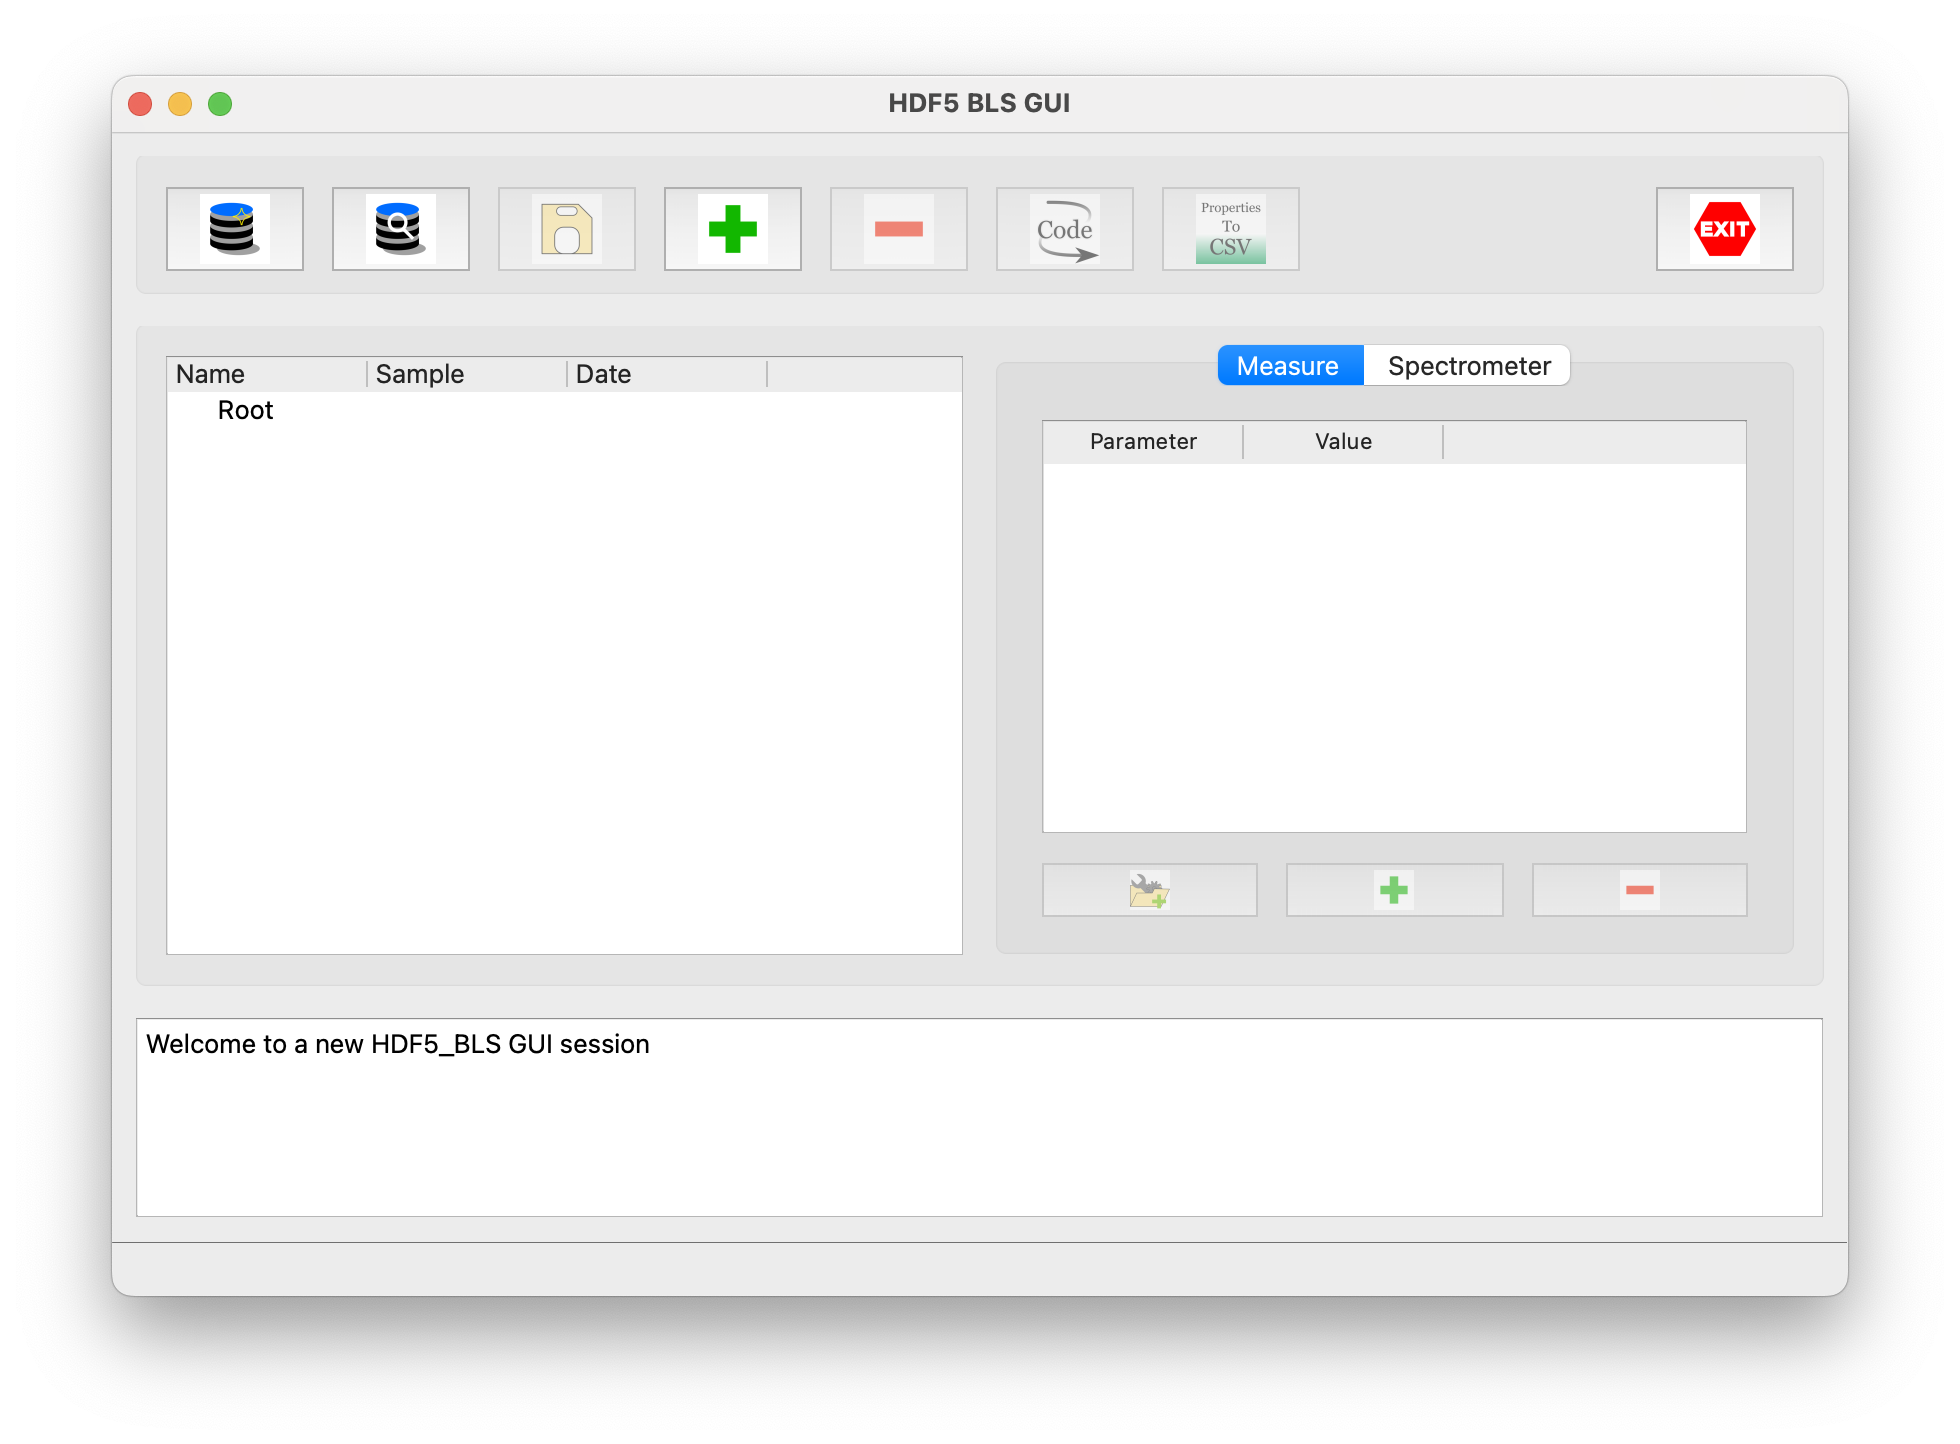
\includegraphics[width=\textwidth]{img/main_window.png}
            \end{center}

            You can then drag and drop your data into the left pannel and structure it as you wish. 
            
            You can also add properties to your data in the form of a standard CSV file which model can be found in the \texttt{spreadsheets} folder of the repository. To add a new property file to your measure, select your measure on the left pannel and drag and drop your property file to the right pannel from a file viewer. 
            
            Note that you can add property to a group of data. In that case, the property apply to all its elements.


\end{document}